%% Included in decks: slidemage-manual
%%

% SlideMage manual, chapter "Accessibility": describing images, with the
% Images tab (tools/manual/make_screenshots.py). The screenshot's own source,
% entered in the Images tab, appears as this slide's automatic
% "Image source:" line.
\begin{standardframe}{Describing images}
	\small
	A reader who cannot see an image needs a description of it. You write each
	description once, in the \emph{Images} tab (Tabs $\rightarrow$ Images), and
	SlideMage puts it into every PDF and transcript that shows the image. A
	local AI model can draft descriptions for you to correct.
	\par\medskip
	\begin{columns}[T,onlytextwidth]
		\begin{column}{0.52\linewidth}
			{\setlength{\fboxsep}{0pt}\fcolorbox{c_primary_gray}{white}{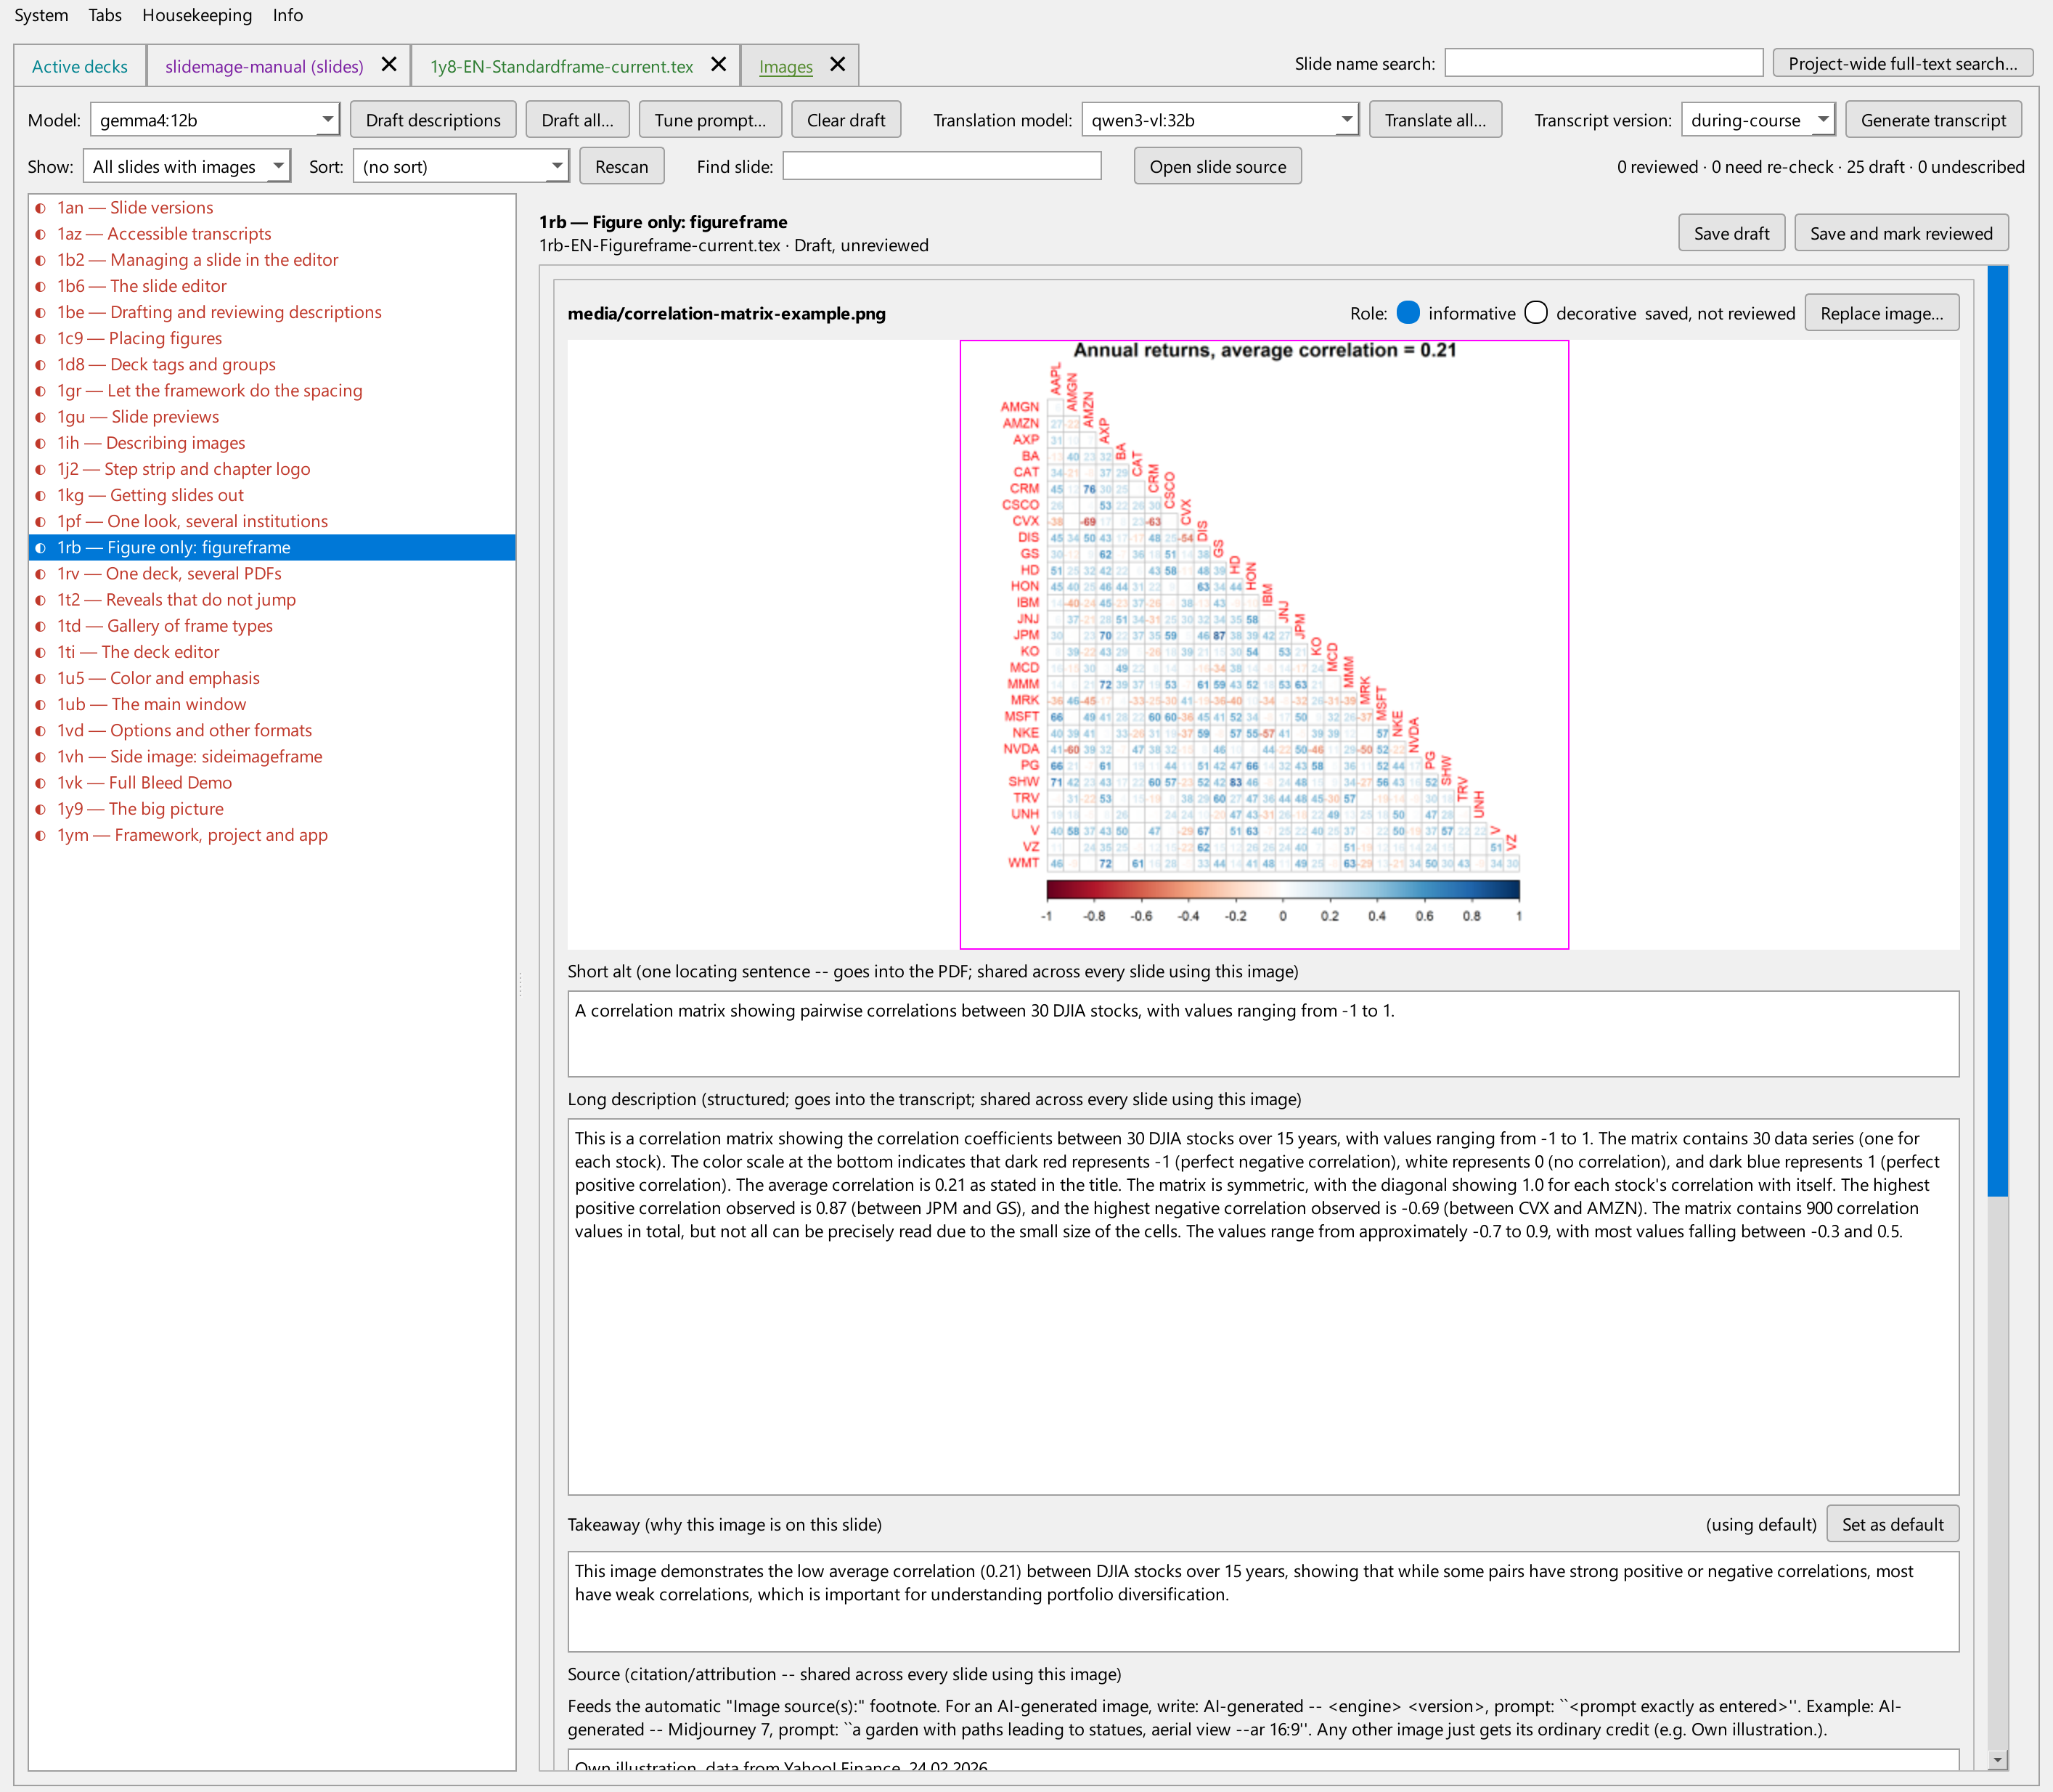
\includegraphics[width=\dimexpr\linewidth-0.8pt\relax]{media/screenshot-slidemage-images-tab.png}}}
		\end{column}
		\begin{column}{0.45\linewidth}
			\shrinklists{1}
			\begin{itemize}
				\item Each image is \emph{decorative} (screen readers skip it) or \emph{informative}: a short and a long description, and a takeaway per slide
				\item Its source, entered once, appears as an \emph{Image source:} line (below)
				\item \emph{Draft all}, \emph{Tune prompt}: drafts by the AI model -- \textbf{check each one}; on faint charts models invent numbers
				\item German fields, with \emph{Translate}
			\end{itemize}
		\end{column}
	\end{columns}
\end{standardframe}
